\documentclass[40pt,a4paper,UTF8]{ctexart}
\usepackage{amsmath}
\usepackage{graphicx}

\usepackage{float}

%输入带圈数字  eg:\textcircled{1}
\usepackage{fontspec,xunicode-addon}

%代码显示的包
\usepackage{listings}
\usepackage{xcolor}

%打出空心字母
\usepackage{amsfonts,amssymb}

%整体加粗
\usepackage{bm}

%公式按照章节标号
\numberwithin{equation}{section}

%长等号
\usepackage{extpfeil}

%列举
\usepackage{enumerate}

%注释用
\usepackage{comment}
%----------------------------------------------
%配置代码显示格式-掌握minted之前的替代品
%----------------------------------------------
\definecolor{codegreen}{rgb}{0,0.6,0}
\definecolor{codegray}{rgb}{0.5,0.5,0.5}
\definecolor{codepurple}{rgb}{0.58,0,0.82}
\definecolor{backcolour}{rgb}{0.95,0.95,0.92}

\lstdefinestyle{mystyle}{
	backgroundcolor=\color{backcolour},   
	commentstyle=\color{codegreen},
	keywordstyle=\color{magenta},
	numberstyle=\tiny\color{codegray},
	stringstyle=\color{codepurple},
	basicstyle=\ttfamily\footnotesize,
	breakatwhitespace=false,         
	breaklines=true,                 
	captionpos=b,                    
	keepspaces=true,                 
	numbers=left,                    
	numbersep=5pt,                  
	showspaces=false,                
	showstringspaces=false,
	showtabs=false,                  
	tabsize=2
}

\lstset{style=mystyle}



%-----------------------------------------------------------------------------------

\title{Motion planning homework 4}
\author{Student name: Francisrk}
\date{Due date: February 13th, 2024}

\begin{document}

\maketitle   %控制序列,能将在导言区中定义的标题、作者、日期按照预定的格式展现出来。


\section{第1题}
\subsection{题目}

- For the OBVP problem stated in slides p.25-p.29, please
get the optimal solution (control, state, and time) for
partially free final state case.

- Suppose the position is fixed, velocity and acceleration
are free here.

\subsection{求解}
首先回顾课程中OBVP如何求解的:
\begin{figure}[H]
\centering
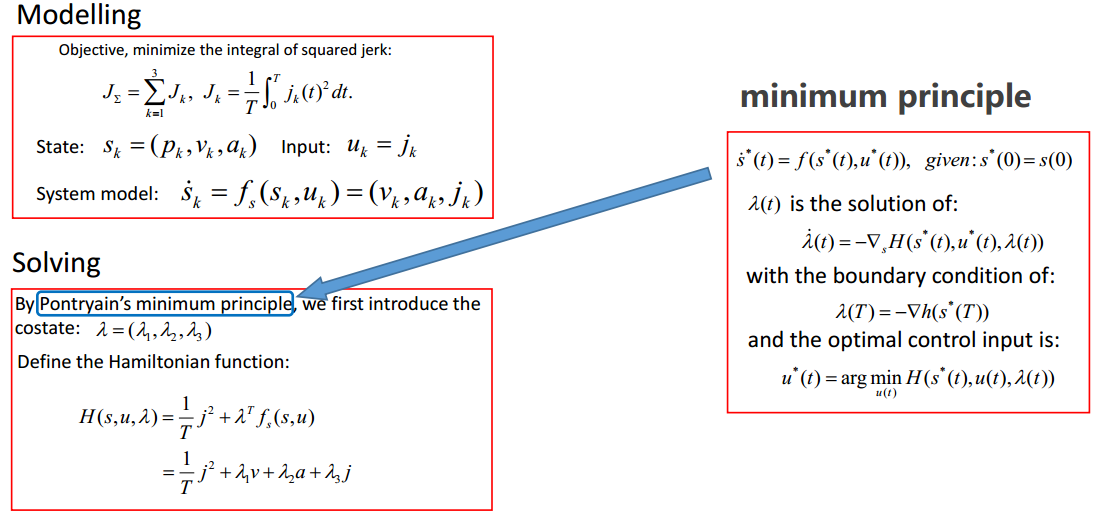
\includegraphics[width=4.8in]{ch4_1.png} {图1.1 四旋翼无人机建模}
\end{figure}

\begin{figure}[H]
\centering
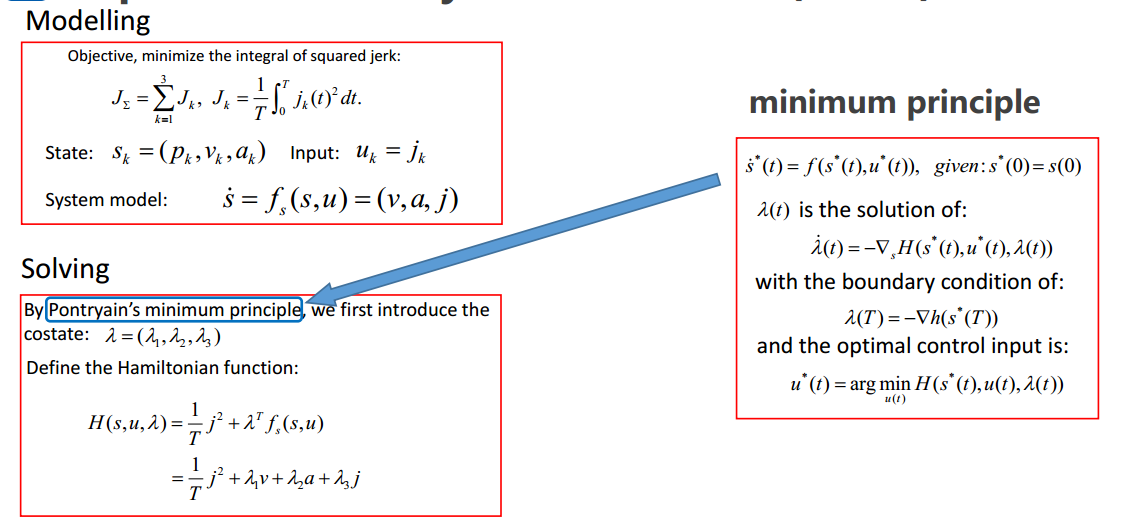
\includegraphics[width=4.8in]{ch4_2.png} {图1.2 对每个轴单独讨论,去掉k}
\end{figure}

\begin{figure}[H]
\centering
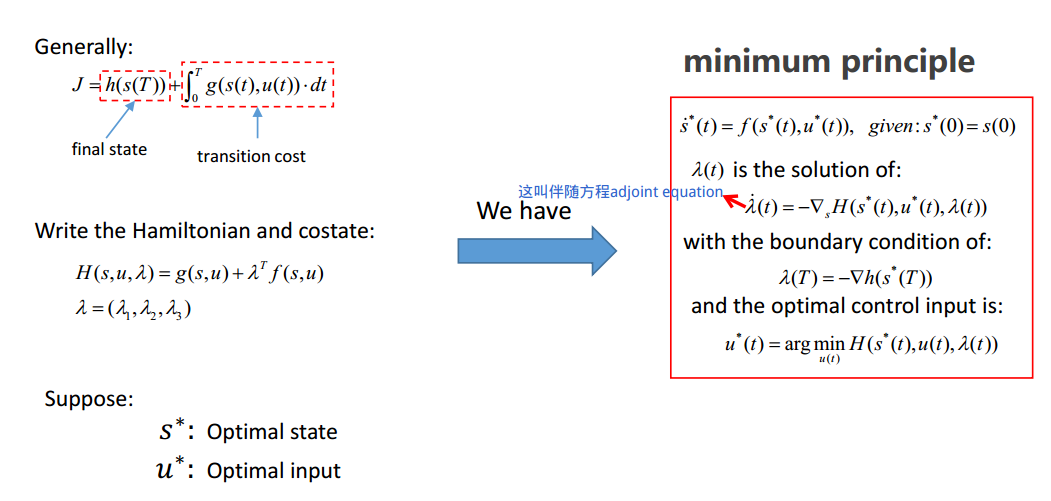
\includegraphics[width=4.8in]{ch4_3.png} {图1.3 引入Pontryain极小值原理,协态变量,Hamiltonian方程}
\end{figure}

\begin{figure}[H]
\centering
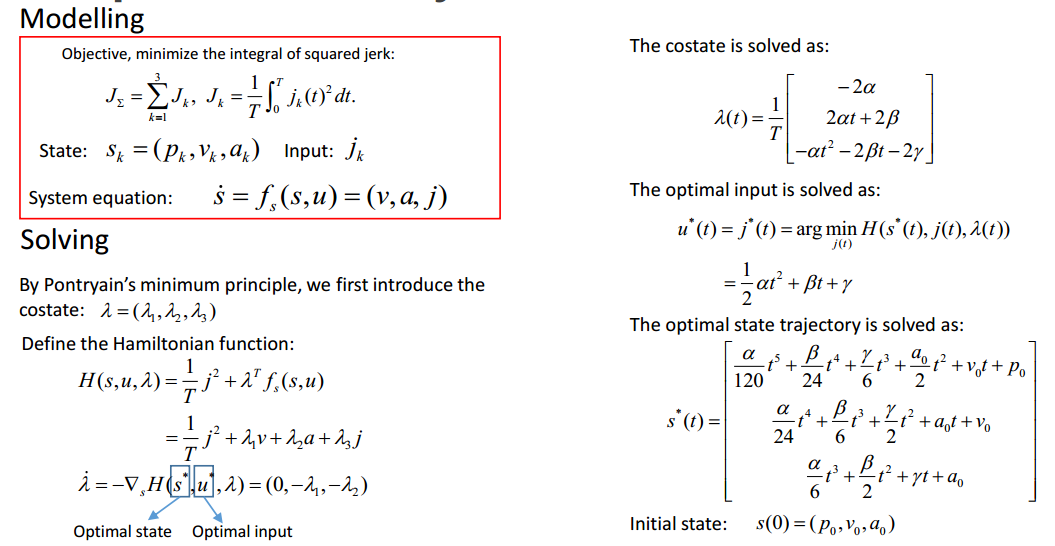
\includegraphics[width=4.8in]{ch4_4.png} {图1.4 求解伴随方程、最优输入、最优状态}
\end{figure}

\begin{figure}[H]
\centering
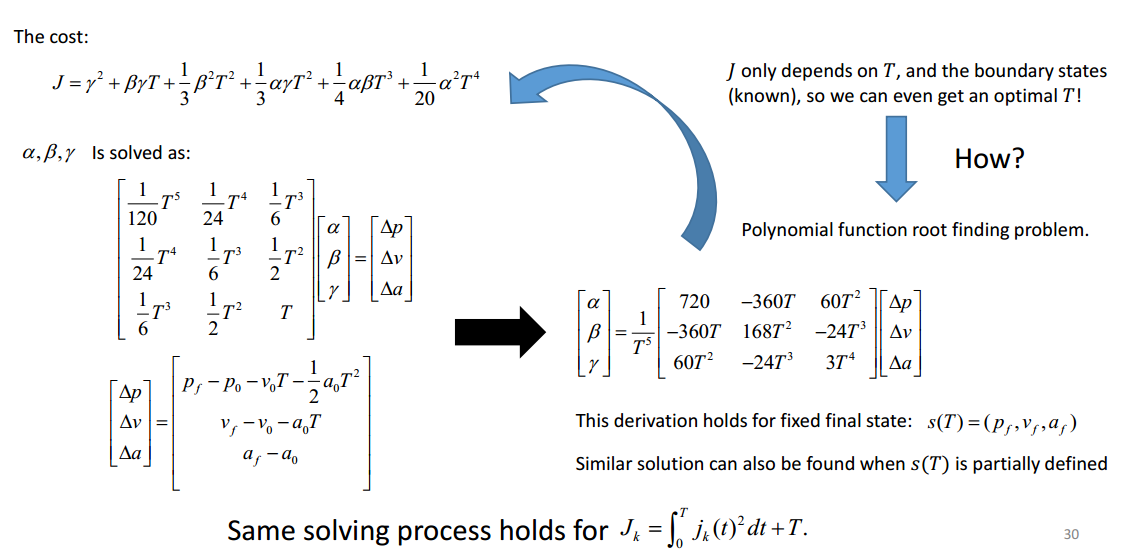
\includegraphics[width=4.8in]{ch4_5.png} {图1.5 根据final state求出协态表达式}
\end{figure}

\begin{figure}[H]
\centering
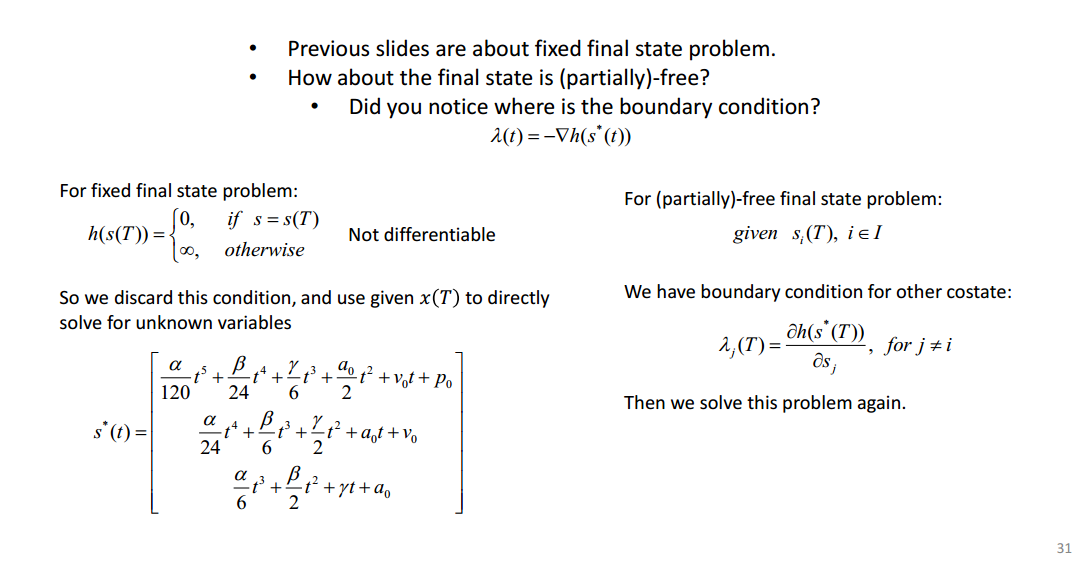
\includegraphics[width=4.8in]{ch4_6.png} {图1.6 讨论final state totally \& partially fixed的情况}
\end{figure}

题目要求最终状态$s^*(T)=(p_f, ?, ?)$,即只fix position,求解此时的OBVP问题,
即求解$u^*(t),s^*(t)$表达式。

为了完整地了解此问题的背景,需要参考该工作的文章\cite{ref1}。

对改文章的前3部分进行简单总结:
本文提出一个用于生成四旋翼运动轨迹生成的一个框架,该框架特点是计算快,易实现。由两个stage组成:
\begin{enumerate}
    \item trajectory generation
    \item feasibilility check
    \end{enumerate}
同时给出了能够保证可行轨迹存在的条件。并在实际的机器上进行了测试。

stage1时无需考虑可行性,所以可快速生成,stage2时由于只需对多项式进行check,所以check速度也很快。

\textbf{1.Introduction部分}

现阶段(2015年)对于四旋翼轨迹生成的研究有两派:
\begin{enumerate}
\item 将几何规划和时域规划解耦。第一步不考虑可行性,进行几何轨迹生成,第二步在时序上进行几何轨迹生成,以保证feasibility。
\item 使用四旋翼动力学的微分平坦性推导出轨迹的约束,并且求解一系列轨迹的优化问题。
\end{enumerate}
本文的方法显然是后者。

现有方法的问题:
\begin{enumerate}
\item 末状态的刚性约束(必须totally fixed)。
\item 末状态可能是时间依赖的(可能流派1的直接解耦不合适)
\item 流派2依赖于凸优化,为了使问题是凸的,可能会减少feasible trajectories的空间。
\end{enumerate}

所以本文主要贡献是:不使用刚性的final state约束,在尽可能大的空间中生成轨迹,然后快速check。

\textbf{2.系统动力学和问题描述部分}

四旋翼被建模为一个9-D的state:$p,v,R$,其中$R$是方向,由于yaw不可观,所以只有8自由度。
系统有3项约束:动力学模型约束,输入约束,仿射平移约束。
由于我们此处只讨论轨迹生成,且本文的算法框架在轨迹生成时不考虑后两种约束,所以对于feasibility check在此处不做讨论,仅考虑动力学约束下的轨迹生成问题。

\textbf{3.运动轨迹生成部分}

同课程所讲相同,系统输入为jerk。需要指出,cost function原本为$f^2||\omega||^2$,但经过推导,其上界为$||j||^2$,所以被积函数为$||j||^2$
对四旋翼的三个轴进行解耦之后,单独讨论每个轴的优化问题,最终推导出$u^*(t)$和$s^*(t)$的closed-form形式:
\begin{align}
j^*(t)&=arg \mathop{min}\limits_{j(t)}H(s^*(t),j(t),\lambda(t)) \notag  \\ 
&=\frac{1}{2}\alpha t^2+\beta t+\gamma
\end{align}


\begin{equation}
s^*(t) = 
\begin{bmatrix}
   \frac{ \alpha}{120}t^5+\frac{\beta}{24}t^4+\frac{\gamma}{6}t^3+\frac{a_0}{2}t^2+v_0t+p_0\\
   \frac{ \alpha}{24}t^4+\frac{\beta}{6}t^3+\frac{\gamma}{2}t^2+a_0t+v_0\\
   \frac{ \alpha}{6}t^3+\frac{\beta}{2}t^2+\gamma t+a_0
\end{bmatrix}
\end{equation}

协态costate
\begin{equation}
    \lambda(t)=\frac{1}{T}
    \begin{bmatrix}
        -2\alpha\\
        2\alpha t+2\beta\\
        -\alpha t^2-2\beta t-2\gamma
    \end{bmatrix}
\end{equation}
其中$\alpha,\beta,\gamma$是需要被确定的,根据final state的约束不同,求解的结果不同,下面将进行讨论。


\begin{enumerate}
\item 当final state totally fixed时,通过带入final state即可求出。该case为rigid constraints,终止terminal condition不再成立,\cite{ref2}中如下图所述:
\begin{figure}[H]
    \centering
    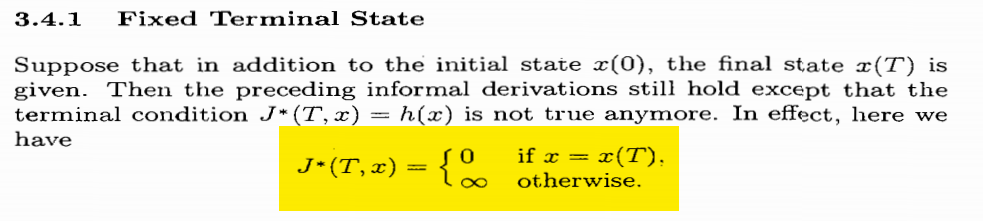
\includegraphics[width=4.8in]{ch4_7.png} {图1.7 当final state totally fixed时,终止条件不成立}
\end{figure}

\item 当final state partially fixed时,仅使用final state的约束无法求解出所有的变量,需要利用boundary condition的约束进行求解。
\cite{ref1}中作者提到“the corresponding costates must equal zero at the end time”,结合\cite{ref2}中的描述
\begin{figure}[H]
    \centering
    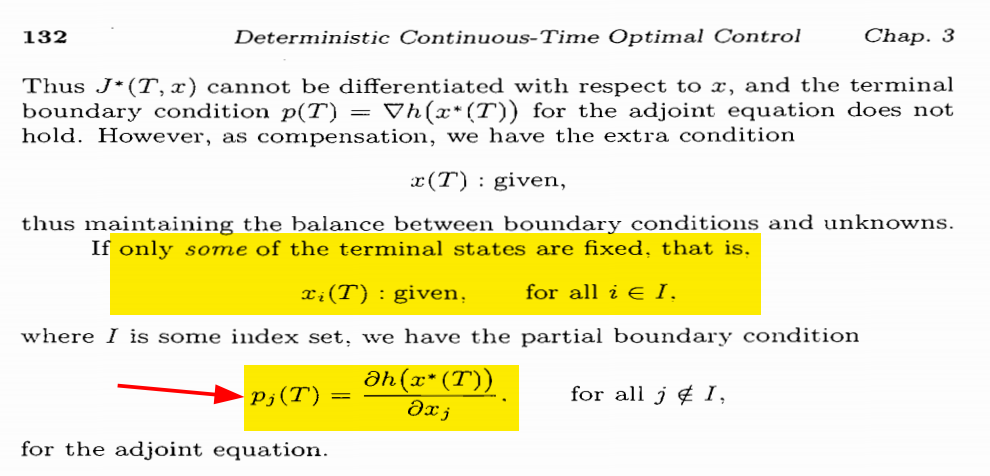
\includegraphics[width=4.8in]{ch4_8.png} {图1.8 final state partially fixed时的boundary condition}
\end{figure}
上图中$p(t)$为costate,也即课程中的$\lambda (t)$,关键结论是

\begin{equation}
    \lambda_j(T)=\frac{\partial{h(s^*(T))}}{\partial{s_j}},for j\neq i
\end{equation}

我们可以得出此时的边界条件,接下来将分别讨论final state中:
\begin{enumerate}
\item only fix $\bm{p_f}$
\item only fix $\bm{v_f}$
\item fix $\bm{p_f, v_f}$
\end{enumerate}
三种情况时的$\alpha,\beta,\gamma$的求解情况。

\begin{enumerate}
\item only fix $\bm{p_f}$时

由boundary condition
\begin{equation}
\left\{
    \begin{array}{l}
    \lambda_2(T)=0\\
    \lambda_3(T)=0
    \end{array}
\right.
\end{equation}

将(1.5)带入(1.3)得
\begin{equation}
\left\{
    \begin{array}{l}
    2 \alpha T+2 \beta=0\\
    -\alpha T^2-2\beta T-2\gamma=0
    \end{array}
\right.
\end{equation}
整理得:
\begin{equation}
    \left\{
        \begin{array}{l}
        \beta=-\alpha T\\
        \gamma = \frac{1}{2}\alpha T^2
        \end{array}
    \right.
\end{equation}

将(1.7)带入(1.2),取第1行整理得
\begin{equation}
\frac{\alpha}{120}T^5 - \frac{\alpha}{24}T^5 +\frac{\alpha}{12}T^5=\Delta p_f
\end{equation}
于是有
\begin{equation}
\alpha = \frac{20}{T^5}\Delta p_f
\end{equation}
将(1.9)带入(1.6),整理得
\begin{equation}
    \begin{bmatrix}
        \alpha \\ \beta \\ \gamma
    \end{bmatrix}
=
\begin{bmatrix}
    \alpha \\ -\alpha T \\ \frac{1}{2}\alpha T^2
\end{bmatrix}
=
\begin{bmatrix}
    1 \\ -T \\ \frac{1}{2}\alpha T^2
\end{bmatrix} \cdot \alpha
=
\begin{bmatrix}
    1 \\ -T \\ \frac{1}{2}\alpha T^2
\end{bmatrix} \frac{20}{T^5}\Delta p_f
=\frac{1}{T^5}
\begin{bmatrix}
    20 \\ -20T \\ 10T^2
\end{bmatrix} \Delta p_f
\end{equation}
此处给出\cite{ref1}附录A中的所有情况的结果
\begin{figure}[H]
    \centering
    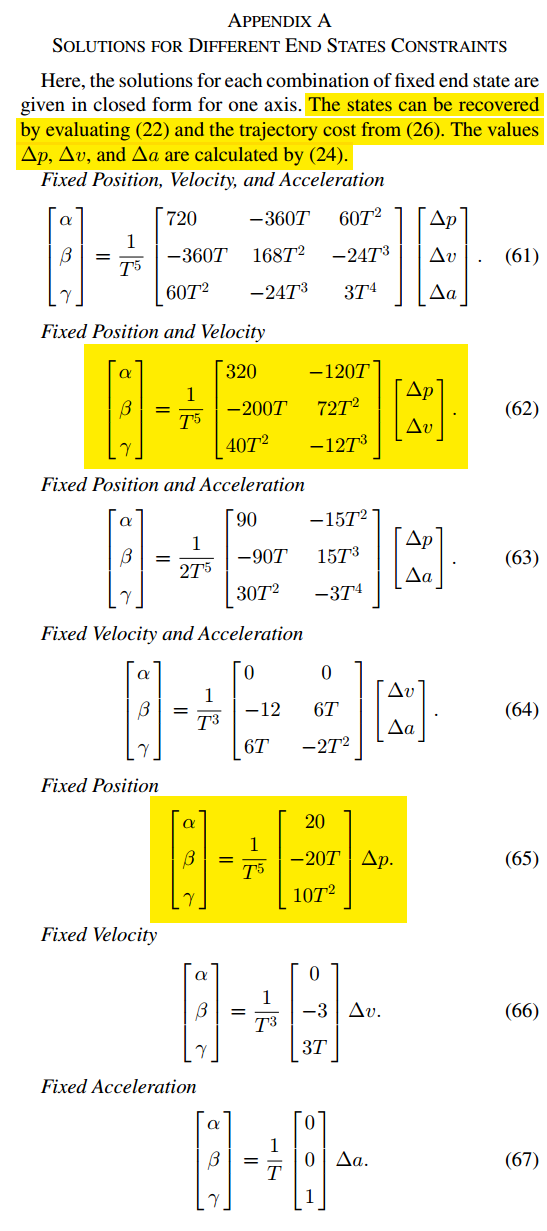
\includegraphics[width=4.8in,height=9.5in]{ch4_9.png} {图4.9 \cite{ref1}Appendix A中当fixed final state不同时的costate结果}
\end{figure}
\item only fix $\bm{v_f}$时

同理,先由(1.4)求得costate约束
\begin{equation}
    \left\{
        \begin{array}{l}
            \alpha = 0\\
            \gamma = -\beta T
        \end{array}
    \right.
\end{equation}
将(1.11)带入(1.2),取第2行得
\begin{equation}
T^3(\frac{-\beta}{3})=\Delta v_f
\end{equation}
则有
\begin{equation}
    \beta = -\frac{3}{T^3}\Delta v_f
\end{equation}
将(1.13)带入(1.11),整理得
\begin{equation}
    \begin{bmatrix}
        \alpha \\ \beta \\ \gamma
    \end{bmatrix}
=
\begin{bmatrix}
    0\\1\\-T
\end{bmatrix}\beta
=
\begin{bmatrix}
    0\\1\\-T
\end{bmatrix}(-\frac{3}{T^3})\Delta v_f
=
\frac{1}{T^3}
\begin{bmatrix}
    0\\-3\\-3T
\end{bmatrix}\Delta v_f
\end{equation}

\item fix $\bm{p_f, v_f}$时

只有$\lambda_3$可以使用boundary condition求得约束,
由(1.4)得costate约束
\begin{equation}
\gamma = -\frac{1}{2}(\alpha T^2 + 2\beta T)
=\begin{bmatrix}
    -\frac{1}{2}T^2 \ -T
\end{bmatrix}
\begin{bmatrix}
    \alpha \\ \beta
\end{bmatrix}
\end{equation}
将(1.15)带入(1.2)整理得
\begin{equation}
    T^5
    \begin{bmatrix}
        -\frac{3}{40}\ -\frac{1}{8T}\\ -\frac{5}{24T}\-\frac{1}{3T^2}
    \end{bmatrix}
    \begin{bmatrix}
        \alpha \\ \beta
    \end{bmatrix} 
    =
    \begin{bmatrix}
        \Delta p_f \\ \Delta v_f
    \end{bmatrix} 
\end{equation}
则有
\begin{equation}
    \begin{bmatrix}
        \alpha \\ \beta
    \end{bmatrix}  
    = \frac{1}{T^5}
    \begin{bmatrix}
        320 \ -120T \\ -200T \ 72T^2
    \end{bmatrix}
    \begin{bmatrix}
        \Delta p_f\\ \Delta v_f
    \end{bmatrix}
\end{equation}
将(1.17)带入(1.15)并与(1.17)联立,整理得
\begin{equation}
    \begin{bmatrix}
        \alpha \\ \beta \\ \gamma
    \end{bmatrix}
    =
    \frac{1}{T^5}
    \begin{bmatrix}
        320 \ -120T \\
        -200T \ 72T^2 \\
        40T^2 \ -12T^3
    \end{bmatrix}
    \begin{bmatrix}
        \Delta p_f \\ \Delta v_f
    \end{bmatrix}
\end{equation}
其中(1.16)矩阵的求逆可使用Matlab的符号运算完成,如图1.10所示
\begin{figure}[H]
    \centering
    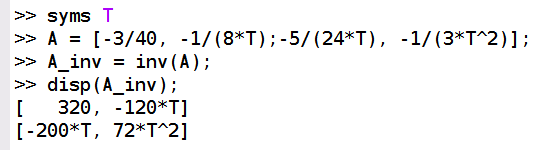
\includegraphics[width=4.8in]{ch4_10.png} {图1.10 使用Matlab完成符号矩阵求逆}
\end{figure}
\end{enumerate}

(1.1)求出$u^*(t)=j^*(t)$之后,带入cost function即可求出cost表达式,
\begin{align}
    J&=\frac{1}{T}\int_{0}^{T}{j_k(t)^2dt} \notag \\
     &=\frac{1}{T}\int_{0}^{T}({\frac{1}{2}\alpha t^2+\beta t+\gamma})dt \notag \\
     &=\frac{1}{20}\alpha^2T^4+\frac{1}{4}\alpha\beta T^3+\frac{1}{3}(\alpha \gamma + \beta^2)T^2 + \beta \gamma T + \gamma^2
\end{align}
由于前面求出的$        \alpha , \beta ,\gamma$均只与$T$相关,所以cost也仅与$T$相关。

需要指出,由于$u^*(t)$是使用Pontryagin极小值原理求得的
通用形式,所以“this cost holds for all combinations of end translational variables”\cite{ref1}


第1题完成。
\end{enumerate}

\subsection{Pontryagin Minimum Principle的拓展}
\begin{figure}[H]
    \centering
    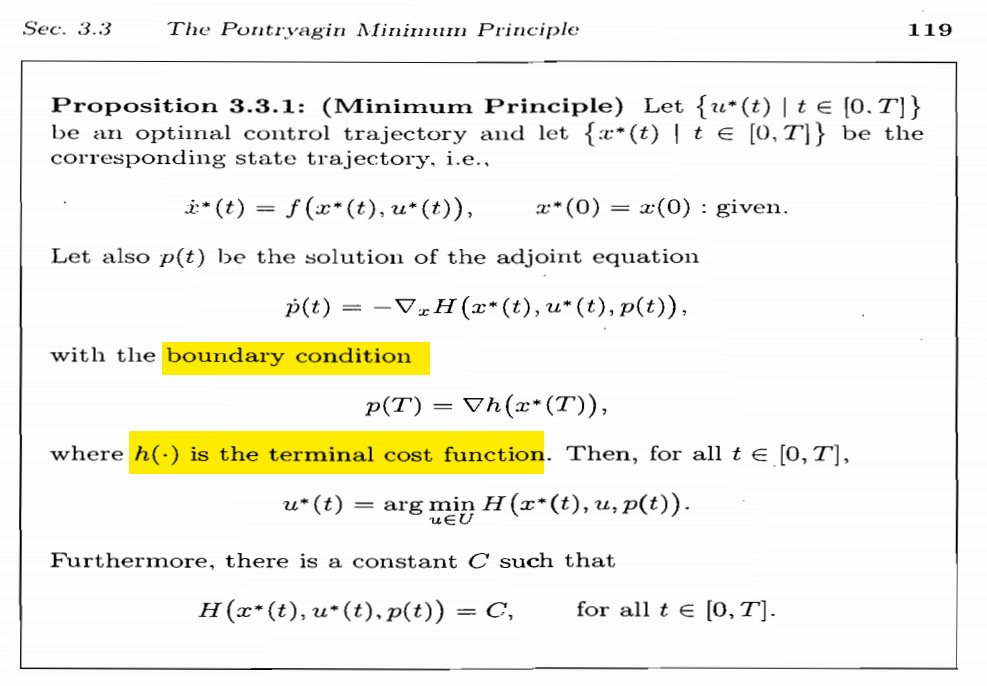
\includegraphics[width=4.8in]{ch4_12.png} {图1.11 Pontryagin Minimum Principle\cite{ref1}}
\end{figure}
以\cite{ref1}中的一个例子来强调adjoint equation和一阶微分方程的求解。
关于一个线性二次问题,
\begin{figure}[H]
    \centering
    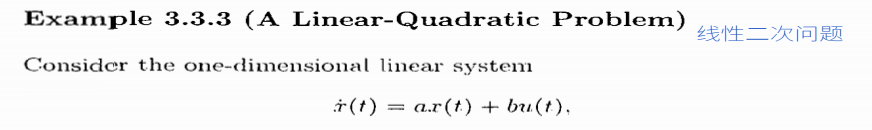
\includegraphics[width=4.8in]{ch4_11.png} {图1.12 linear-quadratic problem\_1\cite{ref1}}
\end{figure}
\begin{figure}[H]
\centering
    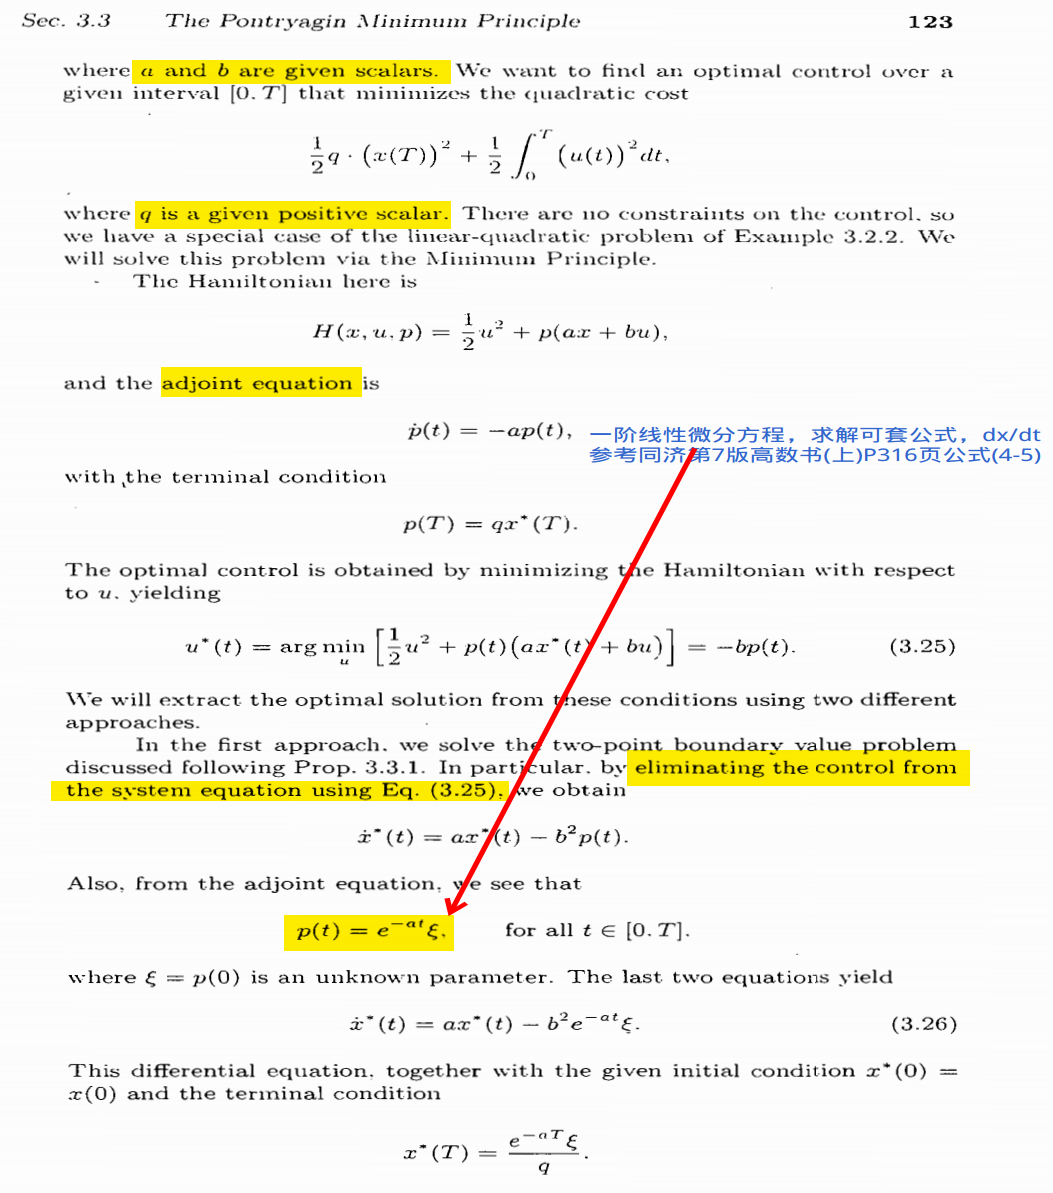
\includegraphics[width=4.8in]{ch4_13.png} {图1.13 linear-quadratic problem\_2\cite{ref1}}
\end{figure}

\begin{figure}[H]
\centering
    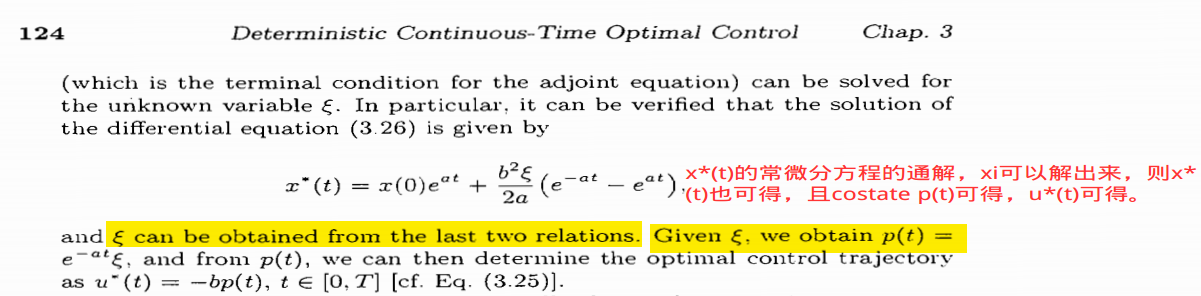
\includegraphics[width=4.8in]{ch4_14.png} {图1.14 linear-quadratic problem\_3\cite{ref1}}
\end{figure}
图1.13中,伴随方程实际上就是课程中解出$\lambda$的微分方程,一阶微分方程求解方式可直接套用公式。
对于形如(1.19)类型的微分方程,可以使用式(1.20)的公式求通解,借助边界条件来求特解。
\begin{equation}
    \frac{dy}{dx}+P(x)y=Q(x)
\end{equation}

\begin{equation}
    y=e^{-\int{P(x)dx}}(\int{Q(x)e^{\int{P(x)dx}}dx+C})
\end{equation}
由图1.12中(3.25)的微分方程整理得:
\begin{equation}
    \frac{d(p(t))}{dt}+ap(t)=0    
\end{equation}
对应(1.19)得$P(x)=a,Q(x)=0$,使用(1.20)得
\begin{equation}
    p(t)=e^{-\int{adt}}(\int{0dt+C}) = e^{-at}C
\end{equation}
令$C=\xi$,则有
\begin{equation}
    p(t)=e^{-at}\xi
\end{equation}
由图1.12中(3.26)的微分方程整理得:
\begin{equation}
    \frac{dx}{dt}-ax =-b^2e^{-at}\xi
\end{equation}
其中$P(x)=-a,Q(x)=-b^2\xi e^{-at}$
使用公式(1.20)求得costate约束
\begin{align}
    x^*(t) &= e^{-\int{(-a)dt}}(\int{-b^2\xi e^{-at}e^{\int{-a dt}}dt}+C)    \notag \\
    &=e^{at}(\frac{b^2\xi}{2a}e^{-2at}+C)
\end{align}
有初始条件
\begin{equation}
    x^*(0)=x(0)
\end{equation}
带入(1.25)得
\begin{equation}
    x(0)=\frac{b^2\xi}{2a}+C
\end{equation}
则
\begin{equation}
    C=x(0)-\frac{b^2\xi}{2a}
\end{equation}
\begin{align}
    x^*(t) &=e^{at}(\frac{b^2\xi}{2a}e^{-2at}+x(0)-\frac{b^2\xi}{2a}) \notag \\
    &=x(0)e^{at}+\frac{b^2\xi}{2a}(e^{-at}-e^{at})
\end{align}
有终止条件
\begin{equation}
    x^*(T)=\frac{e^{-aT}\xi}{q}
\end{equation}
带入(1.29)得
\begin{equation}
    \frac{e^{-aT}\xi}{q} = e^{aT}(\frac{b^2\xi}{2a}e^{-2aT}+x(0)-\frac{b^2\xi}{2a})
\end{equation}
由(1.32)可解出$\xi$,可得$x^*(t)$关于$T$的通解,且costate $p(t)$可得,$u^*(t)$可得,整个系统都可求解。

以上即为Pontryagin Minimum Principle的拓展,主要强调adjoint equation和一阶微分方程的求解方法,更多细节参考\cite{ref2}。

\section{第2题}

\subsection{题目}
Local Lattice Planner

- Build an ego-graph of the linear modeled robot.

- Select the best trajectory closest to the planning target.

\subsection{求解}
\textbf{理论推导部分}

已经给出的建模和求解如图2.1和图2.2所示
\begin{figure}[H]
    \centering
    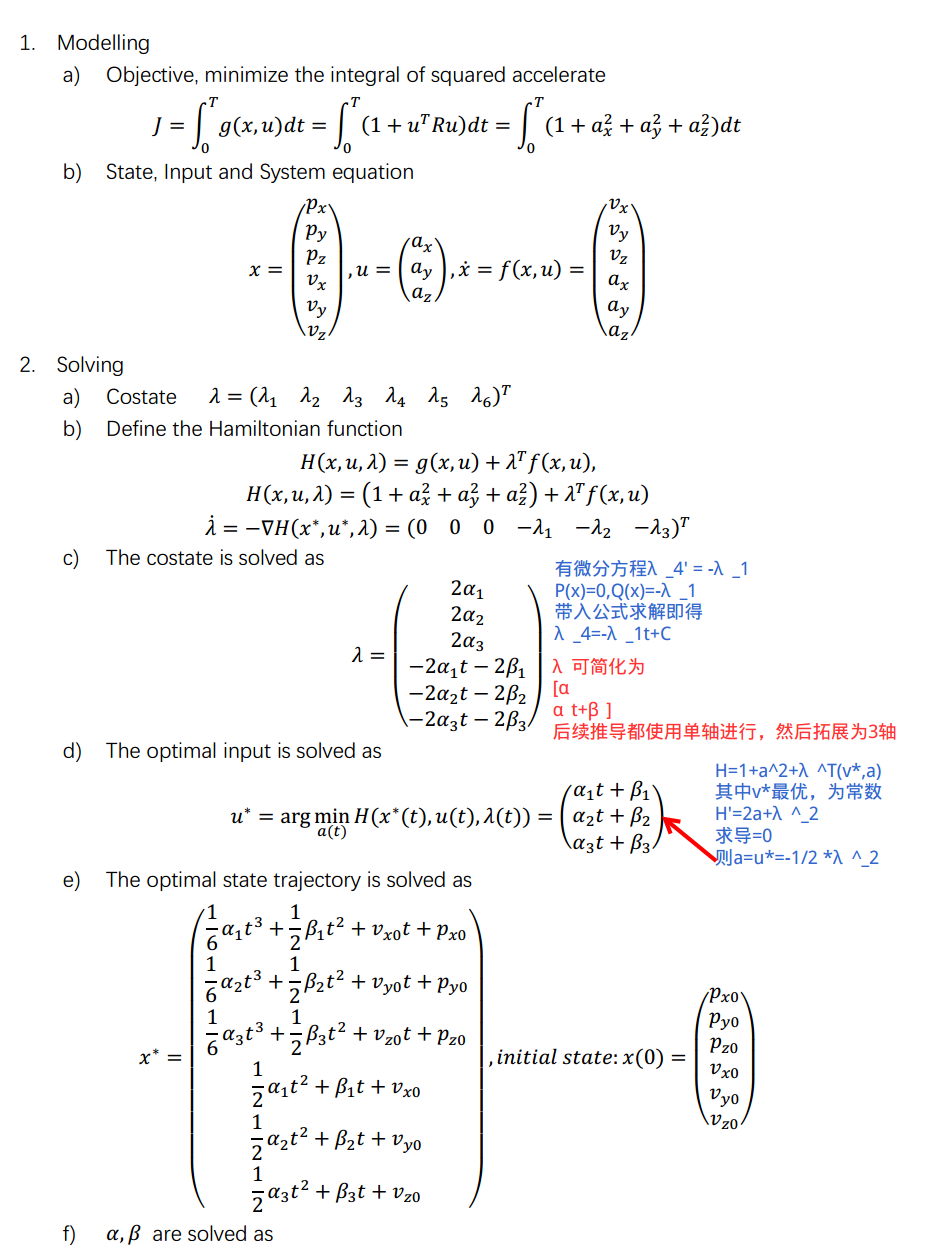
\includegraphics[width=4.8in]{ch4_16.png} {图2.1 建模\&求解\_1}
\end{figure}

\begin{figure}[H]
\centering
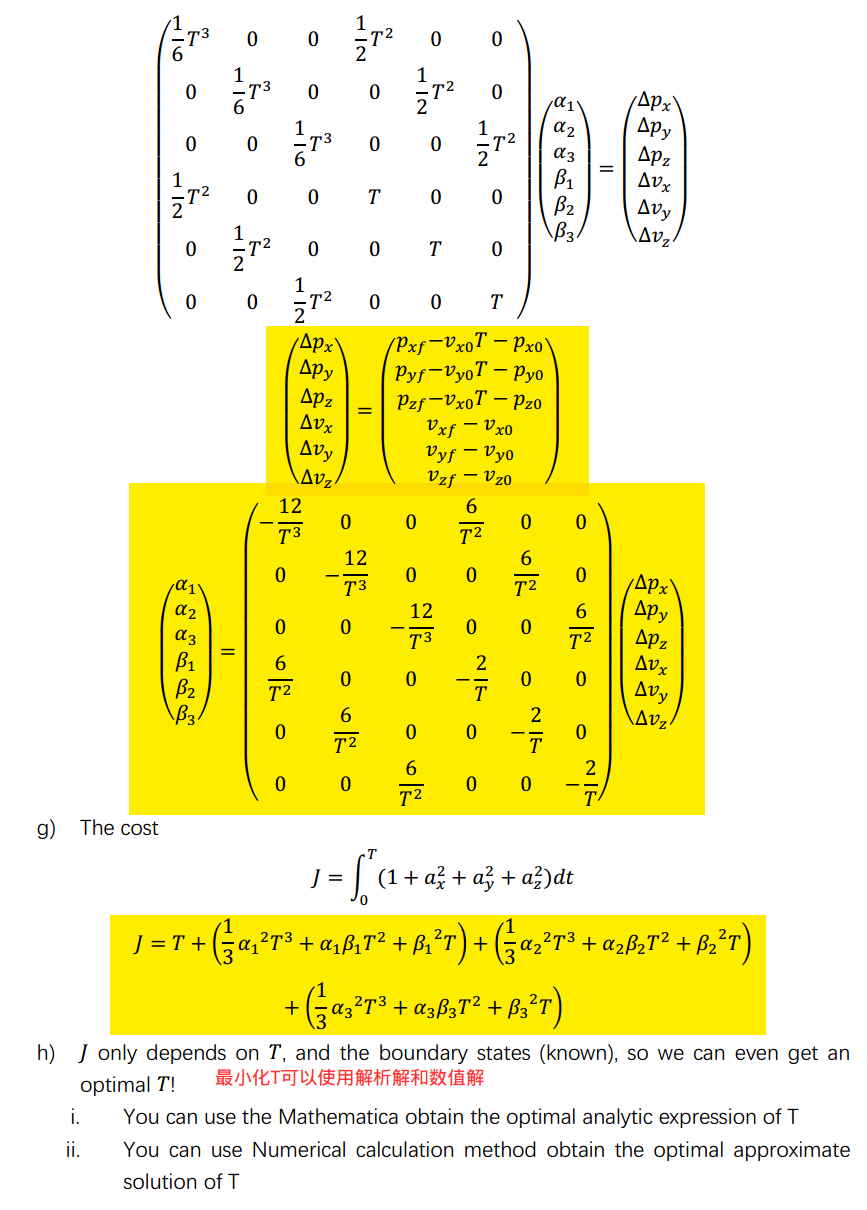
\includegraphics[width=4.8in]{ch4_17.png} {图2.2 建模\&求解\_2}
\end{figure}

系统输入为$u(t)=a(t)$

根据助教的讲解,这里可以把final state中的速度看做常量,在推导过程中直接假设final state中速度为0,
即$v_{xf}=v_{yf}=v_{zf}=0$(这里还不知道为什么可以看做常量)。

所给推导中考虑了三个轴的情况,为了简化,可以只推导单轴情况再拓展为3轴,则对于costate有
\begin{equation}
    \left\{
        \begin{array}{l}
            \alpha = -\frac{12}{T^3}\Delta p +\frac{6}{T^2}\Delta v\\
            \beta = \frac{6}{T^2}\Delta p -\frac{2}{T}\Delta v
        \end{array}
    \right.
\end{equation}

其中
\begin{equation}
    \left\{
        \begin{array}{l}
            \Delta p = p_f - p_0 -v_0T=d_x-v_0T\\
            \Delta v = v_f - v_0 = -v_0
        \end{array}
    \right.
\end{equation}

根据前面推导
\begin{equation}
    J = T+\frac{1}{3}\alpha^2T^3+\alpha\beta T^2 + \beta^2T
\end{equation}

将(2.2)带入(2.1)得
\begin{equation}
    \left\{
        \begin{array}{l}
            \alpha = -\frac{12}{T^3}d_x +\frac{6}{T^2}v_0\\
            \beta = \frac{6}{T^2}d_x -\frac{4}{T}v_0
        \end{array}
    \right.
\end{equation}

整理(2.3)中各项可得
\begin{equation}
    \left\{
        \begin{array}{l}
            \frac{1}{3}\alpha^2T^3 = \frac{48}{T^3}d_x^2 -\frac{48}{T^2}v_0 d_x +\frac{12}{T}v_0^2\\
            \alpha\beta T^2 = -\frac{72}{T^3}d_x^2 +\frac{84}{T}v_0d_x-\frac{24}{T}v_0^2\\
            \beta^2 T=\frac{36}{T^3}d_x^2 -\frac{48}{T^2}v_0d_x+\frac{16}{T}v_0^2
        \end{array}
    \right.
\end{equation}
将(2.5)带入(2.3)得
\begin{equation}
    J=T + \frac{12}{T^3}d_x^2 - \frac{12}{T^2}v_0d_x+\frac{4}{T}v_0^2
\end{equation}
此时cost J只跟T有关,根据Pontryagin Minimum Principle,要对J进行最小化,对J求导等于0
\begin{equation}
    \frac{\partial J}{\partial T} = 0
\end{equation}
最终整理为(2.8)所示的一元四次方程:
\begin{equation}
    T^4-4v_0^2T^2+24v_0d_xT-36d_x^2=0
\end{equation}
方程拓展为三维为:
\begin{align}
    T^4-4(v_{x0}^2+v_{y0}^2+v_{z0}^2)T^2+24(v_{x0}d_x+v_{y0}d_y+v_{z0}d_z)T \notag \\
    -36(d_x^2+d_y^2+d_z^2)=0
\end{align}
式(2.6)cost拓展为三维为
\begin{align}
    J=T + \frac{4(v_{x0}^2+v_{y0}^2+v_{z0}^2)}{T} -
     \frac{12(v_{x0}d_x+v_{y0}d_y+v_{z0}d_z)}{T^2}\notag \\
     +\frac{12(d_x^2+d_y^2+d_z^2)}{T^3}
\end{align}
求解(2.9)可得T,带入(2.10)求得cost,取cost最小的T,且check collision-free即可完成求解。
其中,求解一元四次方程可参考\cite{ref3}

这里采用了方法二,使用多项式的伴随矩阵进行求解:
对于多项式
\begin{equation}
    P(x)=x^n+c_{n-1}x^{n-1}+c_{n-2}x^{n-2}+\cdots +c_1x+c_0
\end{equation}
其伴随矩阵为:
\begin{equation}
    M_x = 
    \begin{bmatrix}
        0 & 0 & \cdots & 0& -c_0 \\
        1 & 0 & \cdots & 0& -c_1 \\
        0 & 1 & \cdots & 0& -c_2 \\
        \cdots & \cdots & \cdots & \cdots & \cdots\\
        0 & 0& \cdots & 1 & -c_{n-1}
    \end{bmatrix}
\end{equation}
其中,$M_x$的特征值就是$P(x)$的根。
所以这里构造的伴随矩阵为
\begin{equation}
    \begin{bmatrix}
        0&0&0&36(d_x^2+d_y^2+d_z^2)\\
        1&0&0&-24(v_{x0}d_x+v_{y0}d_y+v_{z0}d_z)\\
        0&1&0&4(v_{x0}^2+v_{y0}^2+v_{z0}^2)\\
        0&0&1&0
    \end{bmatrix}
\end{equation}


\textbf{代码部分}

STEP1主要使用运动学公式
\begin{equation}
    \left\{
    \begin{array}{l}
    p=p_0+v_0t+\frac{1}{2}at^2\\
    v=v_0+at
    \end{array}
    \right.
\end{equation}
代码如Listing1所示。
\begin{lstlisting}[language=C++, caption=demo\_node.cpp/trajectoryLibrary()]
for(int step=0 ; step<=_time_step ; step ++){
    /*
    STEP 1: finish the forward integration, the modelling has been given in the document
    the parameter of forward integration: _max_input_acc|_discretize_step|_time_interval|_time_step   all have been given
    use the pos and vel to recored the steps in the trakectory
    */
    //使用运动学公式:x=x0+v0t+1/2at^2,v=v0+at
    //要体现出积分,是accumulate的过程
    pos(0) = pos(0) + vel(0) * delta_time + 0.5 * acc_input(0) * std::pow(delta_time, 2);
    pos(1) = pos(1) + vel(1) * delta_time + 0.5 * acc_input(1) * std::pow(delta_time, 2);
    pos(2) = pos(2) + vel(2) * delta_time + 0.5 * acc_input(2) * std::pow(delta_time, 2);
    vel(0) = vel(0) + acc_input(0) * delta_time;
    vel(1) = start_velocity(1) + acc_input(1) * delta_time;
    vel(2) = start_velocity(2) + acc_input(2) * delta_time;

    Position.push_back(pos);
    Velocity.push_back(vel);
    double coord_x = pos(0);
    double coord_y = pos(1);
    double coord_z = pos(2);
    //check if if the trajectory face the obstacle
    if(_homework_tool->isObsFree(coord_x,coord_y,coord_z) != 1){
        collision = true;
    }
}
\end{lstlisting}

STEP2主要构造(2.13)所述的伴随矩阵求根$T$,取出实部为正的最小cost,代码如Listing2所示。
\begin{lstlisting}[language=C++, caption=hw\_tool.cpp/OptimalBVP()]
double Homeworktool::OptimalBVP(Eigen::Vector3d _start_position,Eigen::Vector3d _start_velocity,Eigen::Vector3d _target_position)
{
    double optimal_cost = 1000000; // this just to initial the optimal_cost, you can delete it
    /*
    STEP 2: go to the hw_tool.cpp and finish the function Homeworktool::OptimalBVP
    the solving process has been given in the document

    because the final point of trajectory is the start point of OBVP, so we input the pos,vel to the OBVP

    after finish Homeworktool::OptimalBVP, the Trajctory_Cost will record the optimal cost of this trajectory

    */
    //直接求解一元四次方程

    Eigen::Matrix<double,4,4> mat44;
    Eigen::Matrix<complex<double>, Eigen::Dynamic, Eigen::Dynamic> matrix_eigenvalues;
    //求出一元四次方程的五个系数abcde
    double v_x0 = _start_velocity(0), v_y0 = _start_velocity(1), v_z0 = _start_velocity(2);

    double dx = _target_position(0) - _start_position(0);
    double dy = _target_position(1) - _start_position(1);
    double dz = _target_position(2) - _start_position(2);
    double v0_square_sum = v_x0*v_x0 + v_y0*v_y0 + v_z0*v_z0;
    double v0_dp_sum = v_x0*dx+v_y0*dy+v_z0*dz;
    double dp_square_sum = dx*dx + dy*dy + dz*dz;

    double a = 1.0;
    double b = 0.0;
    double c = -4 * v0_square_sum;
    double d = 24 * v0_dp_sum;
    double e = -36 * dp_square_sum;

    mat44 <<
            0, 0, 0, -e,
            1, 0, 0, -d,
            0, 1, 0, -c,
            0, 0, 1, -b;
//    ROS_INFO_STREAM("\nmatrix_44: \n" << mat44);
    matrix_eigenvalues = mat44.eigenvalues();
//    ROS_INFO_STREAM("\nmatrix_eigenvalues: \n"<<matrix_eigenvalues);

    for(int i=0; i<4; ++i) {
        if(matrix_eigenvalues(i).real() < 0)
            continue;
        double T = matrix_eigenvalues(i).real();
        double tmp_cost = T + 4.0/T * v0_square_sum - 12.0/(std::pow(T,2)) * v0_dp_sum + 12.0/std::pow(T,3) * dp_square_sum;
        ROS_INFO_STREAM("\nnow optimal_cost=" << optimal_cost <<", tmp_cost= " << tmp_cost);
        if(tmp_cost < optimal_cost) {
            ROS_INFO_STREAM("\n======now optimal_cost=" << optimal_cost <<", found lower cost= " << tmp_cost);
            optimal_cost = tmp_cost;
        }
    }
    ROS_INFO_STREAM("\nreturn optimal_cost=" << optimal_cost);
    return optimal_cost;
}
\end{lstlisting}

最终运行结果如图2.3所示,其中green for optimal trajectory,red for not collision-free trajectory,
blue for collision-free trajectory.
\begin{figure}[H]
    \centering
    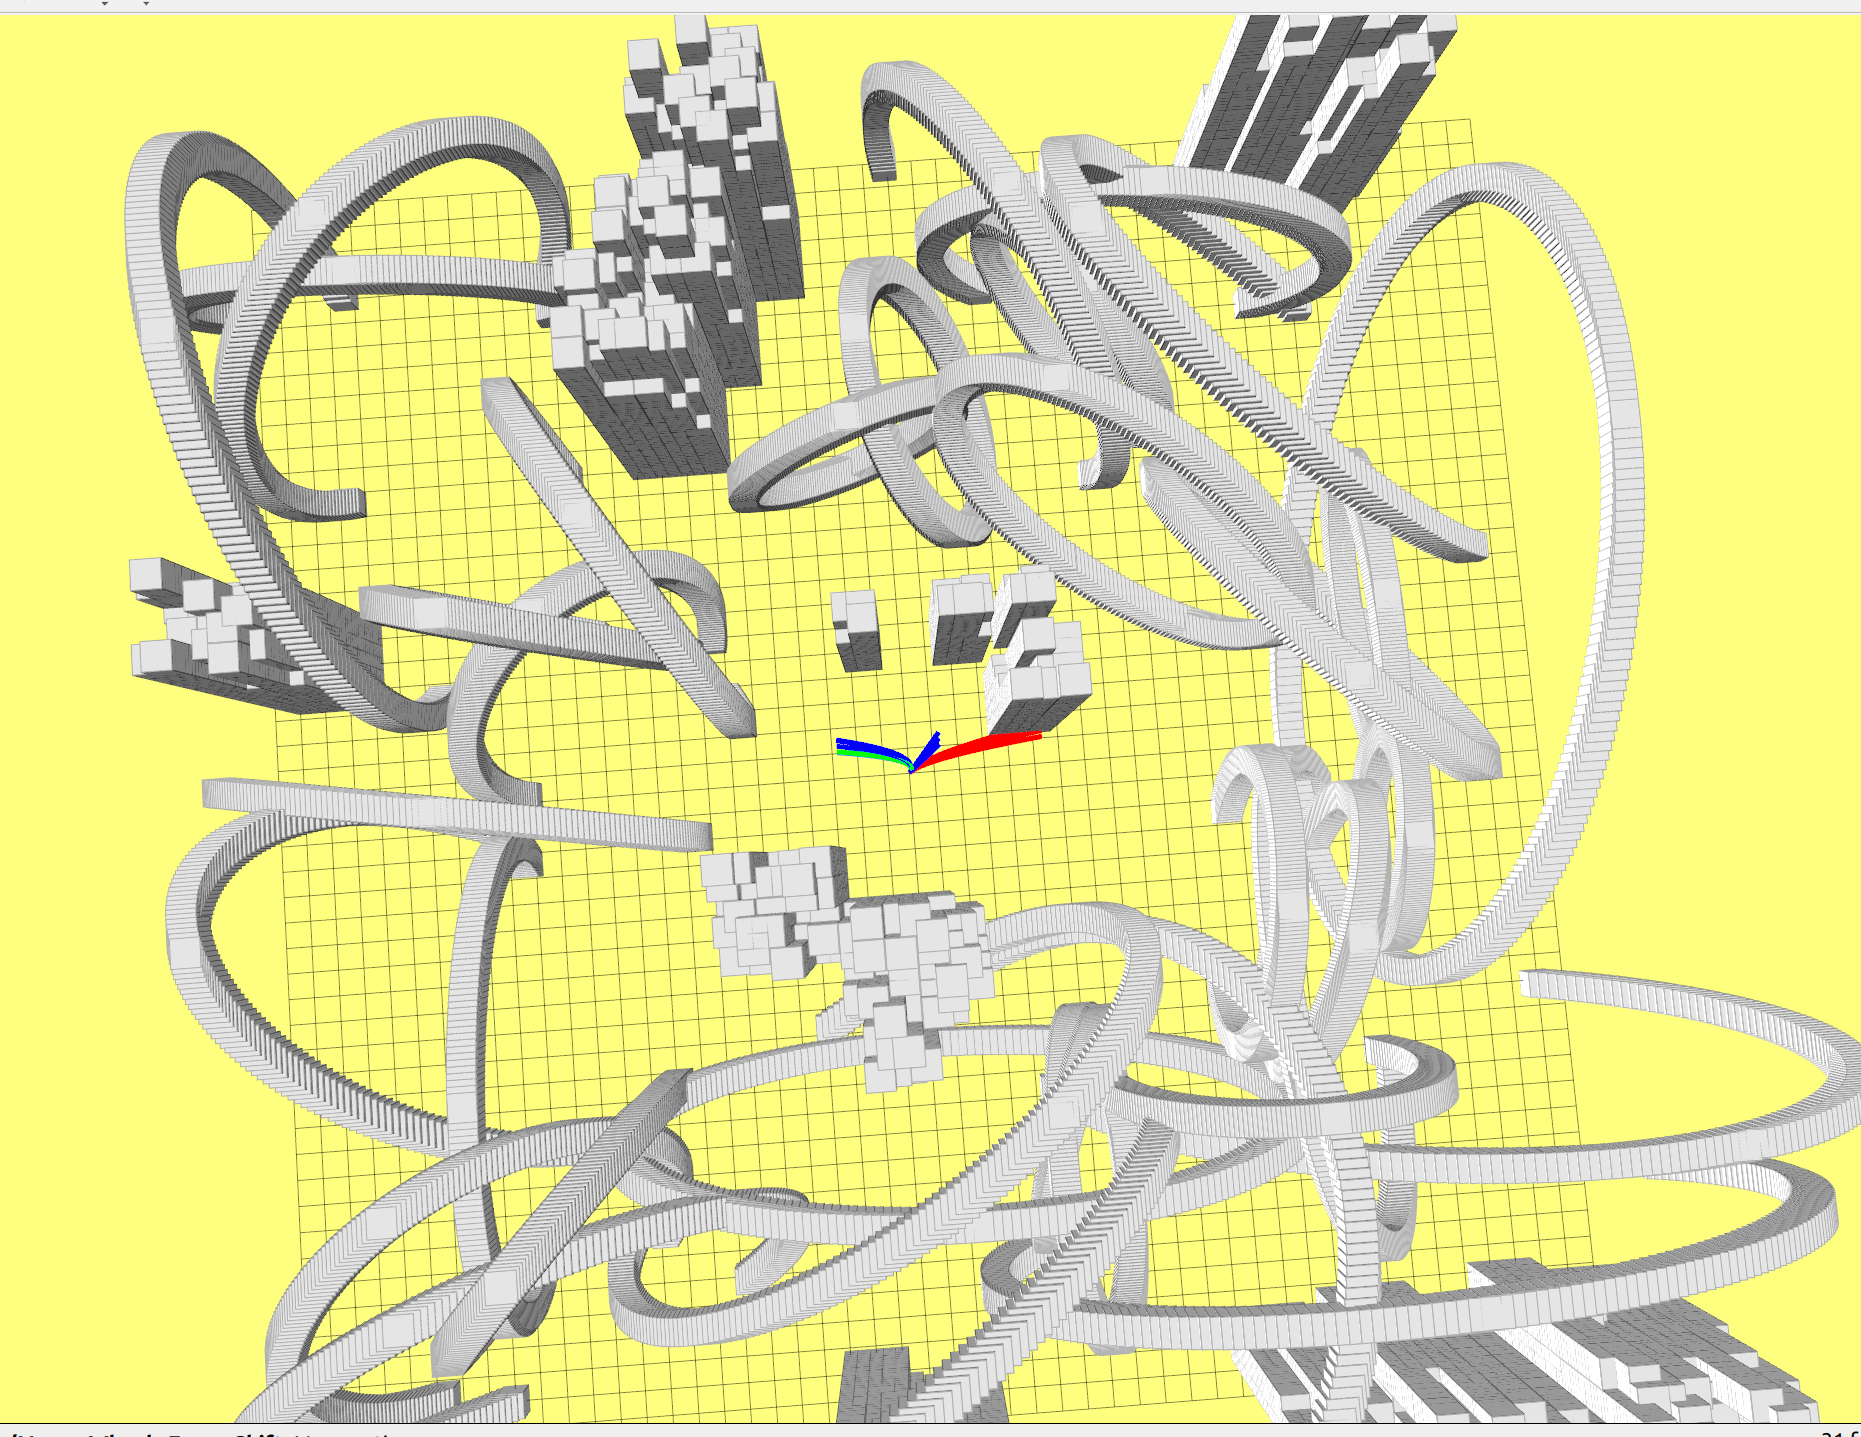
\includegraphics[width=4.8in]{ch4_15.png} {图2.3 运行结果}
\end{figure}


\begin{thebibliography}{99}  
\bibitem{ref1}A Computationally Efficient Motion Primitive for Quadrocopter Trajectory Generation, Mark W. Mueller, Markus Hehn, and Raffaello D’Andrea.
\bibitem{ref2}Dynamic Programming and Optimal Control, D. P. Bertsekas.
\bibitem{ref3}https://blog.csdn.net/fb\_941219/article/details/102984587
\end{thebibliography}




\end{document}